\section{Creación de una infraestructura de red de tarjetas Zybo}
\hypertarget{CreacionInfraestructura}{}
\subsection{Material necesario}
Para la creación de la infraestructura de red física de placas Zybo contaremos con el siguiente material:
\begin{itemize}
	\item Placas Zybo Zynq-7010.
	\item Un ordenador con sistema operativo Linux (Debian 9 Stretch)\footnote{También es posible usar cualquier otra distribución de Linux.} y Windows 7.
	\item Un switch tp-link modelo TL-SG1024D.
	\item Software Vivado.
\end{itemize}

%\newpage
\subsubsection{Placas Zybo Zynq-7000}
\begin{figure}[h]
	\centering
	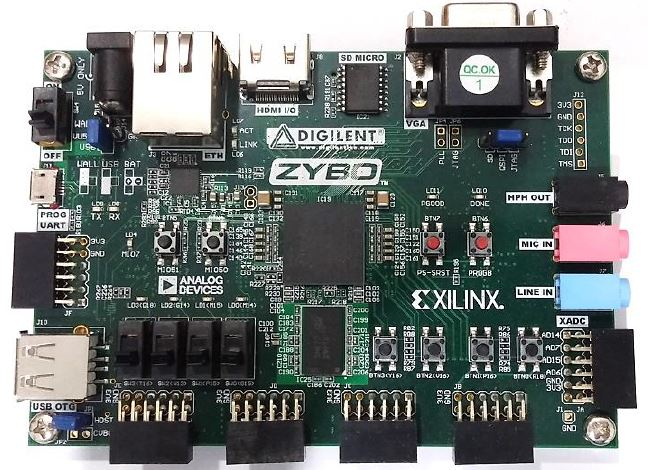
\includegraphics[scale=0.5]{Anexos/Anexo2/Infraestructura/zybo.jpg}
	\caption{Placa Zybo Zynq 7010}
	\label{Placa Zybo}
\end{figure}
Para este proyecto necesitaremos poder programar la FPGA integrada en la placa desde la tarjeta SD de memoria. Para ello se va a preparar una imagen para que el procesador ARM integrado en la placa arranque desde la tarjeta SD y pueda programar la FPGA. El sistema operativo elegido es Linux.

Las placas Zybo Zynq 7010 tienen tres posibles modos de arranque que podemos seleccionar con el jumper JP5: QSPI, SD, JTAG. En este proyecto, el sistema operativo estará en la tarjeta SD, por lo tanto, tendremos que cambiar el jumper JP5 (situado arriba a la derecha) a la posición ``SD''\footnote{Dicho jumper está identificado con el número 21 en la imagen de la siguiente página.}.

\newpage
\begin{figure}[h]
	\centering
	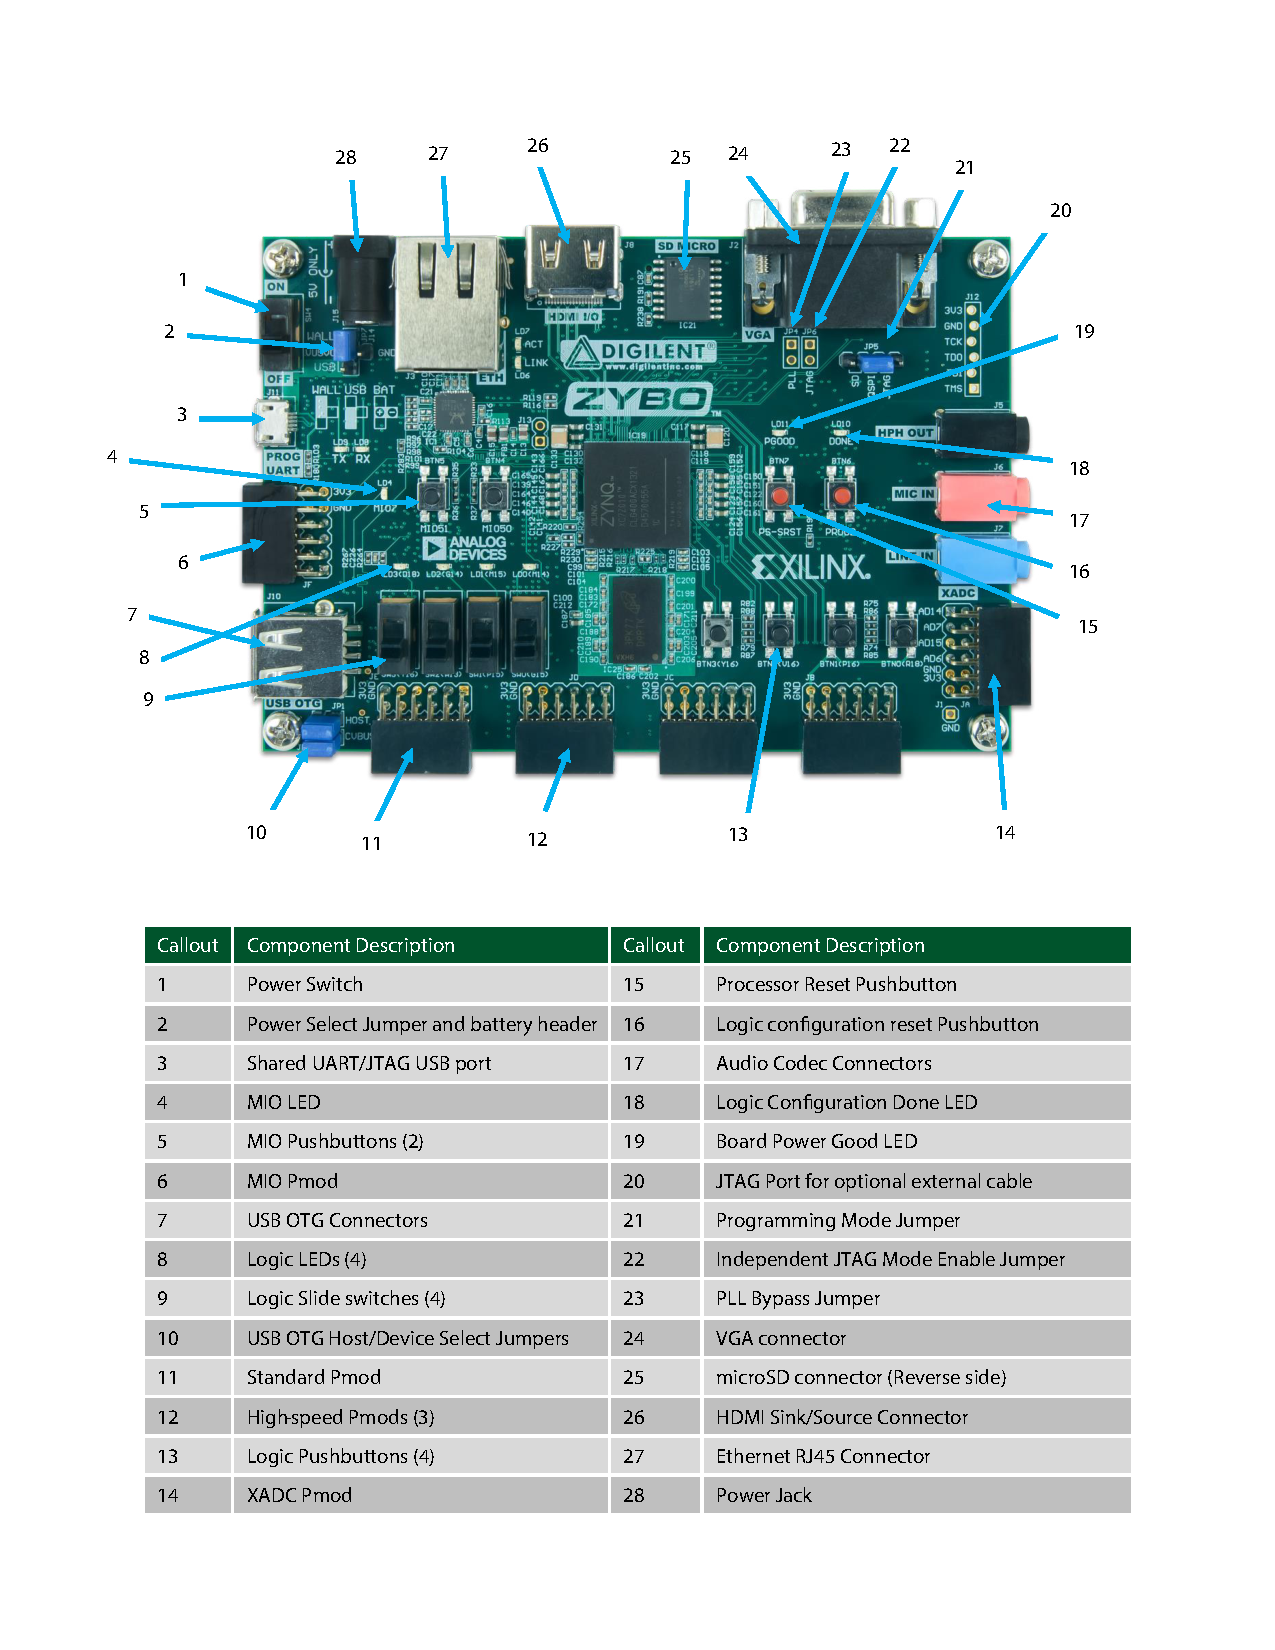
\includegraphics[scale=0.69]{Anexos/Anexo2/Infraestructura/Datasheet.pdf}
	\caption{Diagrama de Zybo Zynq 7010 procedente del manual de referencias}
	\label{Diagrama de Zybo Zynq 7010 procedente del manual de referencias}
\end{figure}
\begin{center}
	\textbf{Fuente:} Manual de referencia oficial de \href{https://reference.digilentinc.com/_media/zybo:zybo_rm.pdf}{\textcolor{blue}{DIGILENT$^{\circledR}$}}.
\end{center}

\newpage
\subsubsection{Ordenador central}
\begin{itemize}
	\item \textbf{Sistemas operativos:} El ordenador usado en el proyecto tendrá dos sistemas operativos.
	\begin{itemize}
		\item \textbf{Debian 9 Stretch:} Este sistema operativo tendrá un usuario llamado \texttt{zybo} y su contraseña será \texttt{zybomonitor}. La contraseña para los permisos de super-usuario también será \texttt{zybomonitor}. Este sistema operativo realizará la clonación del sistema operativo Linux a partir de la imagen generada en el Trabajo de Fin de Grado de Gabriel Fernando Sánchez Reina \hyperlink{2}{[2]}.
	\end{itemize}

	\item \textbf{Red:} El ordenador central tendrá dos interfaces de red:
	\begin{itemize}
		\item \textbf{Red externa:} Interfaz que nos proporcionará acceso a Internet en el ordenador central mediante la red de la UCA.
		\item \textbf{Red interna:} Interfaz conectada al switch del proyecto y tendrá la IP 192.168.1.10 (estática).
	\end{itemize}
\end{itemize}


\subsubsection{Switch}
El switch usado en este proyecto es el modelo tp-link TL-SG1024D que cuenta con 24 puertos con tecnología Gigabit y conectores RJ-45. También cuenta con interfaz accesible para su configuración.


\subsection{Pasos para el montaje de la infraestructura}
\subsubsection{Asignar direcciones IP}
Para asignarles las direcciones de IP a los dispositivos diferenciamos entre:
\begin{itemize}
	\item \textbf{Ordenador:} Debemos identificar la interfaz de red con la que estamos trabajando. Para ello, abrimos un terminal y ejecutamos el siguiente comando como super-usuario\footnote{Comando \texttt{su} y contraseña \texttt{zybomonitor}.}:
	\begin{center}
		\texttt{ifconfig}
	\end{center}
	\newpage
	\begin{figure}[h]
		\centering
		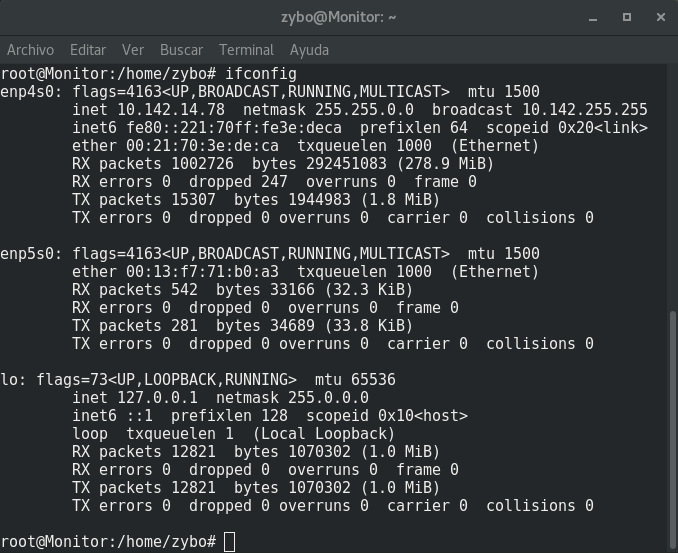
\includegraphics[scale=0.5]{Anexos/Anexo2/Infraestructura/ifconfigPC.png}
		\caption{Interfaces de red del ordenador central}
		\label{Interfaces de red del ordenador central}
	\end{figure}
	
	En la figura \ref{Interfaces de red del ordenador central}, podemos ver las siguientes interfaces:
	\begin{itemize}
		\item \textbf{enp4s0:} Interfaz de red externa.
		\item \textbf{enp5s0:} Interfaz de red interna.
	\end{itemize}
	
	Una vez identificada la interfaz, debemos acceder al fichero\\ \texttt{/etc/network/interfaces.d/INTERFAZ}\footnote{Siendo \texttt{INTERFAZ}, la interfaz que estamos usando. En este ejemplo, \texttt{enp5s0}.} como super-usuario con el siguiente comando:
	\begin{center}
		\texttt{gedit /etc/network/interfaces.d/enp5s0}
	\end{center}
	Y lo modificamos de la siguiente forma:
	\begin{lstlisting}
	allow-hotplug enp5s0
	    iface enp5s0 inet static
	    address 192.168.1.10
	    netmask 255.255.255.0
	    gateway 192.168.1.1
	\end{lstlisting}
	
	\newpage
	\item \textbf{Tarjetas Zybo:} Conectamos la tarjeta mediante USB al ordenador y abrimos un terminal serie en PuTTY\footnote{Puerto ttyUSB1 y velocidad 115200.} e iniciamos sesión en Linux\footnote{Usuario: \texttt{zyboX}; contraseña \texttt{zyboX}. Siendo \texttt{X} el identificador de la tarjeta.}.
	
	\begin{figure}[h]
		\centering
		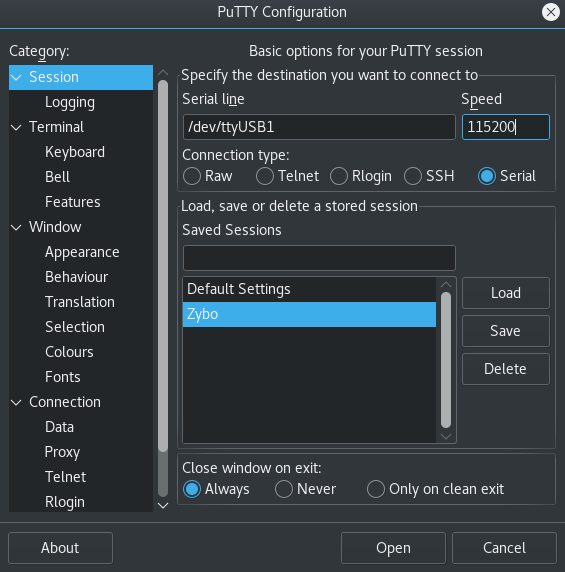
\includegraphics[scale=0.7]{Anexos/Anexo2/Infraestructura/PuTTY.png}
		\caption{Configuración de PuTTY}
		\label{Configuración de PuTTY}
	\end{figure}
	
	Debemos identificar la interfaz de red con la que estamos trabajando. Para ello, ejecutamos el siguiente comando como super-usuario\footnote{Comando \texttt{su} y contraseña \texttt{root}.}:
	\begin{center}
		\texttt{ifconfig}
	\end{center}
	\newpage
	\begin{figure}[h]
		\centering
		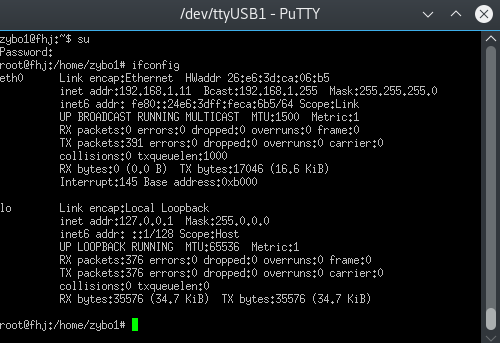
\includegraphics[scale=0.8]{Anexos/Anexo2/Infraestructura/ifconfigZybo.png}
		\caption{Interfaces de red de la tarjeta Zybo}
		\label{Interfaces de red de la tarjeta Zybo}
	\end{figure}
	
	Una vez identificada la interfaz, debemos acceder al fichero\\ \texttt{/etc/network/interfaces.d/INTERFAZ}\footnote{Siendo \texttt{INTERFAZ}, la interfaz que estamos usando. En este ejemplo \texttt{eth0}.} como super-usuario con el siguiente comando:
	\begin{center}
		\texttt{nano /etc/network/interfaces.d/eth0}
	\end{center}
	Y lo modificamos de la siguiente forma:
	\begin{lstlisting}
	allow-hotplug eth0
	    iface eth0 inet static
	    address 192.168.1.11
	    netmask 255.255.255.0
	    gateway 192.168.1.1
	\end{lstlisting}
	\newpage
	Para establecer la dirección IP del resto de dispositivos, repetiremos el proceso y estableceremos las direcciones IP siguiendo la siguiente tabla:
	\begin{table}[h]
		\centering
		\begin{tabular}{|c|c|}
			\hline
			\textbf{Dispositivo} & \textbf{Dirección IP} \\ \hline
			Monitor & 192.168.1.10 \\ \hline
			Zybo1 & 192.168.1.11 \\ \hline
			Zybo2 & 192.168.1.12 \\ \hline
			Zybo3 & 192.168.1.13 \\ \hline
			Zybo4 & 192.168.1.14 \\ \hline
		\end{tabular}
		\caption{Direcciones IP de las tarjetas}
		\label{Direcciones IP de las tarjetas}
	\end{table}
	
	Las tarjetas estarán identificadas como ZyboX (siendo ``X'' el identificador de la tarjeta con la que estamos trabajando) y el ordenador se identificará como ``Monitor''.
	
	Se puede observar que el número identificador de la tarjeta coincide con el último número de la dirección IP $- 10$, de tal forma que si queremos añadir la tarjeta \texttt{Zybo10}, su dirección IP será 192.168.1.20.
\end{itemize}


\subsubsection{Conexión al switch de las placas Zybo}
Una vez tengamos los dispositivos identificados tenemos que conectarlos al switch\footnote{Podemos conectar los dispositivos al puerto del switch que queramos debido a que se encargará de ir rellenando su tabla CAM con las direcciones de los dispositivos que tiene conectados.}. No es necesario una configuración previa del switch ni entrar en su interfaz web, ya que no vamos a requerir acciones avanzadas.

Para probar la conectividad entre todos los dispositivos tendremos que ejecutar el test de interconexión de red. Dicho test se encuentra descrito en el anexo \hyperlink{TestConexion}{Test de interconexión de red Zybo}. 